\documentclass{book}

\usepackage[UTF8]{ctex}
\usepackage{graphicx}
\usepackage{booktabs}
\usepackage{enumerate}
\usepackage{xurl}
\usepackage{xcolor}
\usepackage{scrtime}
\usepackage{setspace}
\usepackage[font={bf,stretch=1}]{caption}
\usepackage{makeidx}
\usepackage{menukeys}
\usepackage{threeparttable}
\usepackage{array}
\usepackage{subfigure}
\usepackage[noautomatic]{imakeidx}
\usepackage{hyperref}


\hypersetup{colorlinks}
\makeindex[intoc]

\title{戴森球计划手册}
\author{HuangFuSL}

\ifx\commitId\undefined
    \providecommand{\commitId}{草稿}
\fi

\newcommand{\objimg}[2]{\includegraphics[height=1.5cm]{./imgs/#2/#1.png}}
\newcommand{\itemimg}[1]{\objimg{#1}{items}}
\newcommand{\techimg}[1]{\objimg{#1}{techs}}
\newcommand{\buildingimg}[1]{\objimg{#1}{buildings}}
\newcommand{\upgradeimg}[1]{\objimg{#1}{upgrades}}
\newcommand{\starimg}[1]{\objimg{#1}{stars}}
\newcommand{\planetimg}[1]{\objimg{#1}{planets}}

\setstretch{1.5}
\renewcommand\arraystretch{1.25}

\begin{document}
    \begin{titlepage}
        \begin{center}
            \vspace*{1cm}
    
            \textbf{\Huge 戴森球计划手册}
                
            \vspace{1.5cm}
    
            \textsc{\Large HuangFuSL}
    
            \vfill
                
            \textsc{https://github.com/DSP-Handbook/DSP-Handbook}

            \commitId 版本编译于\today\thistime
                
        \end{center}

    \end{titlepage}
    \tableofcontents
    %! TEX root = ./main.tex
\chapter{游戏任务及目标}
    %! TEX root = ./main.tex
\chapter{星系与天体}

\label{chap:spheres}

\section*{单位设定}

游戏中的单位换算关系如表\ref{tbl:unit-conversion}所列,功率、能量、时间等其他单位的换算关系与SI单位制相同:

\begin{table}[h]
    \centering
    \small
    \caption{单位换算关系}
    \begin{tabular}{ccc}
        \toprule
        单位描述 & 单位符号 & 换算关系 \\
        \midrule
        行星单位直径 & $D$ & $400\mathrm m$ \\
        恒星单位半径 & $R\odot$ & $1600\mathrm m$ \\
        天文单位 & AU & $40000\mathrm m$ \\
        光年 & LY & $60\mathrm {AU}$ \\
        \bottomrule
    \end{tabular}
    \label{tbl:unit-conversion}
\end{table}

\section{恒星}

在“新游戏”界面,玩家可以手动选择星系种子,恒星数量与星球资源倍率。星系种子、恒星数量决定了星区中恒星的分布。在游戏中,恒星的参数有质量、光谱类型、半径、光度、表面温度及年龄等。\index{恒星}\index{星系种子}

\subsection{光谱类型}

\index{光谱类型}

恒星共有M、K、G、F、A、B、O等光谱类型,其光度按照此顺序递增。同时,恒星颜色从红色逐渐过渡到黄色、白色直至蓝色(图\ref{fig:color-dist})。此外,白矮星、黑洞、中子星在游戏中同样被视为恒星,它们在游戏内的光谱类型显示为X。除普通恒星外,星系中会少量分布巨星恒星,它们相较于普通恒星有更大的质量和半径。以红巨星、蓝巨星最为常见,黄巨星及白巨星出现的频率较少。红巨星可能的光谱类型包含M、K、G等,蓝巨星可能的光谱类型包含A、B、O等。
\index{白矮星}\index{黑洞}\index{中子星}\index{巨星}

\begin{figure}[htb]
    \centering
    \subfigure[M]{\starimg M}
    \subfigure[K]{\starimg K}
    \subfigure[G]{\starimg G}
    \subfigure[F]{\starimg F}
    \subfigure[A]{\starimg A}
    \subfigure[B]{\starimg B}
    \subfigure[O]{\starimg O}
    \caption{不同光谱类型的恒星}
    \label{fig:color-dist}
\end{figure}

不同光谱类型的恒星在星系中的出现频率不同,B型恒星与G型恒星在星系中出现最为频繁。表\ref{tbl:amount-dist}统计了100个随机星系种子中不同类型恒星的数量分布(恒星数量固定为64)。

\begin{table}[h]
    \centering
    \small
    \caption{恒星数量分布}
    \begin{tabular}{ccccc}
        \toprule
        光谱类型 & 恒星平均数量 & 百分比 & 方差 & $95\%$置信区间 \\
        \midrule
        M & $4.84$ & $7.6\%$ & $3.20$ & $(4.49, 5.19)$ \\
        K & $10.2$ & $16.0\%$ & $6.80$ & $(9.72, 10.7)$ \\
        G & $13.8$ & $21.5\%$ & $7.05$ & $(13.2, 14.3)$ \\
        F & $4.90$ & $7.7\%$ & $2.78$ & $(4.57, 5.23)$ \\
        A & $2.99$ & $4.7\%$ & $2.68$ & $(2.67, 3.31)$ \\
        B & $21.1$ & $33.0\%$ & $2.66$ & $(20.8, 21.6)$ \\
        O & $2.12$ & $3.3\%$ & $1.15$ & $(1.91, 2.33)$ \\
        X & $4.00$ & $6.2\%$ & $0.00$ & $(4.00, 4.00)$ \\
        \bottomrule
    \end{tabular}
    \label{tbl:amount-dist}
\end{table}

恒星的光谱类型决定了其质量、光度及半径分布。除巨星外,O型恒星有最高的质量、最高的光度和最大的半径,M型恒星的质量和半径最小,光度最低。因此,在玩家选择建设戴森球(参见第\ref{chap:dyson-sphere}章)时,通常会选择在O型恒星、B型恒星或蓝巨星的行星上建立戴森球。它们更大的半径意味着可以建立更大的戴森球,更高的光度意味着单位面积戴森球壳可以接收到更多的能量。

\section{行星}

\index{行星}

行星是围绕恒星或巨行星运转的星球。每颗恒星的行星系都会包含1-6颗行星。其中气态巨星或冰巨星也会伴随若干颗卫星生成。

\subsection{类型}

\index{行星!类型}

行星的不同类型会影响其资源分布,游戏中共有如表\ref{tbl:planet-type}所列的22种行星。每个星系中只会有一颗地中海类型的行星且为游戏开始登陆的行星。

\begin{table}[hp]
    \small
    \centering
    \caption{22种行星类型}
    \label{tbl:planet-type}

    \begin{tabular}{
        m{1.5cm}<{\centering} m{1.5cm}<{\centering}
        m{1.5cm}<{\centering} m{1.5cm}<{\centering}
        m{1.5cm}<{\centering} m{1.5cm}<{\centering}
    }
        \toprule
        星球类型 & 星球外观 & 星球类型 & 星球外观 & 星球类型 & 星球外观 \\
        \midrule

        地中海 & \planetimg{M} & 干旱荒漠 & \planetimg{AD} & 灰烬冻土 & \planetimg{AG} \\
        海洋丛林 &  \planetimg{OJ} & 熔岩 & \planetimg{L} & 冰原冻土 & \planetimg{IFG} \\
        贫瘠荒漠 & \planetimg{BD} & 戈壁 & \planetimg{G} & 火山灰 & \planetimg{VA} \\
        红石 & \planetimg{RS} & 草原 & \planetimg{P} & 水世界 & \planetimg{W} \\
        黑石盐滩 & \planetimg{RSL} & 樱林海 & \planetimg{SO} & 飓风石林 & \planetimg{HSF} \\
        猩红冰湖 & \planetimg{SIL} & 热带草原 & \planetimg{S} & 橙晶荒漠 & \planetimg{CD} \\
        极寒冻土 & \planetimg{FT} & 潘多拉沼泽 & \planetimg{PS} & 气态巨星 & \planetimg{GG} \\
        冰巨星 & \planetimg{IG} & & & & \\
        \bottomrule
    \end{tabular}
\end{table}

巨星是一类特殊的行星,此类行星没有陆地或海洋,因此不能放置大多数类型的建筑,机甲也无法降落在巨星上。在游戏中,气态巨星提供氢和重氢两种资源,冰巨星提供可燃冰和氢两种资源。在登陆巨星后,可以手动从行星表面采集资源。研究“气态行星采集”科技后也可以在巨星的赤道上放置轨道采集器以自动化采集资源。使用轨道采集器收集的资源需要使用星际物流运输船转运到星际物流运输站才可供使用。“矿物利用”科技同样适用于轨道采集器,可以提高资源的采集效率,不过巨星上的资源可以无限采集而不会耗尽。

\index{巨星}\index{气态巨星}\index{冰巨星}\index{行星!巨星}

\subsection{运动状态}

\index{行星!运动状态}

在星系中,少数行星会表现出特殊的运动状态,会对星球的日夜更替产生影响。

\begin{enumerate}
    \item \textbf{轨道共振:}行星的公转周期与自转周期成比例,意味着行星的日夜更替更慢;
    \item \textbf{潮汐锁定:}行星的公转周期与自转周期相等,即轨道共振1:1。潮汐锁定导致行星的的一面永远是白昼,另一面永远是黑夜;\index{潮汐锁定}
    \item \textbf{反向自转:}行星的自转方向与普通行星相反;
    \item \textbf{横躺自转:}行星的自转轴和公转平面的夹角小,日夜更替更为复杂;
    \item \textbf{卫星:}行星围绕另一颗行星而非恒星公转。
\end{enumerate}

\subsection{网格结构}

游戏中的所有行星有相同的网格结构。赤道被等分为1000格网格,每条经线被划分为500格网格,从赤道向两极延伸,沿纬线排列的网格数量逐渐减少。具体的网格结构如表\ref{tbl:network-structure}所示。

赤道附近有最大的网格范围($161\times 1000$),因此适合大规模摆放生产线。在摆放建筑时,建筑会自动吸附到网格节点上,按下\keys{Shift}可以取消网格吸附以更加自由地摆放建筑。

\begin{table}[ht]
    \small
    \centering
    \caption{行星网格结构}
    \label{tbl:network-structure}
    \begin{tabular}{cccc}
        \toprule
        层级 & 纬度范围 & 经线方向网格数 & 纬线方向网格数 \\
        \midrule
        赤道 & $0^\circ$ & 1 & 1000 \\
        1 & $0^\circ \sim 28^\circ 48'$ & 80 & 1000 \\
        2 & $28^\circ 48'\sim 46^\circ 48'$ & 50 & 800 \\
        3 & $46^\circ 48'\sim 55^\circ 48'$ & 25 & 600 \\
        4 & $55^\circ 48'\sim 64^\circ 48'$ & 25 & 500 \\
        5 & $64^\circ 48'\sim 70^\circ 12'$ & 15 & 400 \\
        6 & $70^\circ 12'\sim 75^\circ 36'$ & 15 & 300 \\
        7 & $75^\circ 36'\sim 79^\circ 12'$ & 10 & 200 \\
        8 & $79^\circ 12'\sim 82^\circ 48'$ & 10 & 160 \\
        9 & $82^\circ 48'\sim 84^\circ 36'$ & 5 & 100 \\
        10 & $84^\circ 36'\sim 86^\circ 24'$ & 5 & 80 \\
        11 & $86^\circ 24'\sim 88^\circ 12'$ & 5 & 40 \\
        12 & $88^\circ 12'\sim 90^\circ$ & 5 & 20 \\
        \midrule
        总计 & $0^\circ \sim 90^\circ$ & 250 & - \\
        \bottomrule
    \end{tabular}
\end{table}

\section{星图}

在游戏内按下\keys{V}键可以打开星图,在星图界面中可以查看任何恒星、行星的类型、资源分布\marginpar{
    \footnotesize 查看天体的资源分布需要研发“宇宙探索”升级

    \vspace{0.5cm}
    \centering
    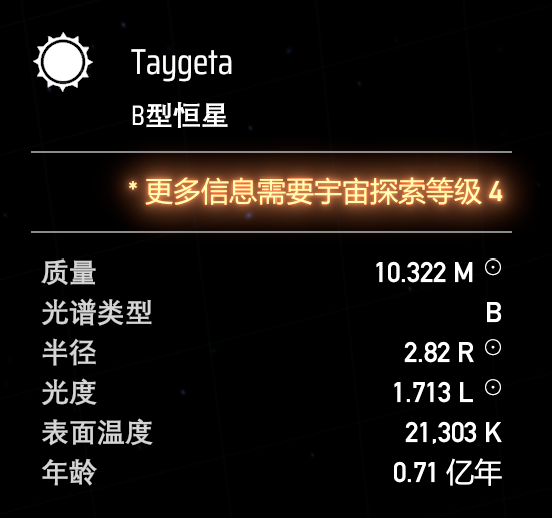
\includegraphics[width=3.5cm]{imgs/screenshots/spheres-info.png}
}及轨道参数。\index{星图}

\section{元数据}

\index{元数据}

0.9.25.11985版本中加入了元数据的设定,每个存档中生产的各种超级矩阵按照每分钟产量分配至元数据中,在其他存档中可以直接提取为超级矩阵或用于研发科技。但若两个存档的星系种子、恒星数量与星球资源倍率完全相同,则\textbf{无法}从该存档中提取元数据。

在创建存档时,设定的星球资源倍率会影响元数据的产出比率,星球的资源倍率越低,单位产量对应的元数据越多。

\begin{table}
    \footnotesize
    \centering
    \caption{行星网格结构}
    \label{tbl:metadata-ratio}
    \begin{tabular}{*{11}{c}}
        \toprule
        资源倍率 & 极少 & 0.5x & 0.8x & 1x & 1.5x & 2x & 3x & 5x & 8x & 无限 \\
        \midrule
        元数据比率 & $400\%$ & $200\%$ & $150\%$ & $100\%$ & $90\%$ & $80\%$ & $70\%$ & $60\%$ & $50\%$ & $40\%$ \\
        \bottomrule
    \end{tabular}
\end{table}
    %! TEX root = ./main.tex
\chapter{物品}
    %! TEX root = ./main.tex
\chapter{建筑}
    %! TEX root = ./main.tex
\chapter{生产线}
    %! TEX root = ./main.tex
\chapter{科技与研发}
    %! TEX root = ./main.tex
\chapter{机甲活动与升级}
    %! TEX root = ./main.tex
\chapter{戴森球}

\label{chap:dyson-sphere}

    \appendix
    %! tex root = ../main.tex

\chapter{许可协议}

除特别标明外,本作品使用CC BY-NC-SA 4.0公共许可协议进行共享。协议全文来自于\url{https://creativecommons.org/licenses/by-nc-sa/4.0/legalcode.zh-Hans}

\begin{center}
    \textbf{\Large 知识共享 (Creative Commons) 署名—非商业性使用—相同方式共享 4.0公共许可协议国际版}
\end{center}

通过行使本协议所授予的权利(定义如下),您接受并同意受到知识共享(Creative Commons)署名—非商业性使用—相同方式共享4.0国际公共许可协议(以下简称“本公共许可协议”)的约束。从合同解释的角度来看,您获得授权的对价是接受本协议的条款,许可人授予您这些权利的对价是可以通过采用本协议条款发布授权作品(material)而获得利益。

\section*{第一条\;定义} \label{section:A.1}

\begin{enumerate}[a.]
    \item \textbf{演绎作品(Adapted Material):} 指受到著作权与类似权利保护的,基于授权作品(Licensed Material)而创作的作品(material),例如对授权作品(Licensed Material)的翻译、改编、编排、改写或其他依据著作权与类似权利需要获得所有人许可的修改。为本公共许可协议之目的,当授权作品(Licensed Material)为音乐作品、表演或录音时,将其依时间序列关系与动态影像配合一致而形成的作品,视为演绎作品(Adapted Material)。\label{entry:A.1.a}
    \item \textbf{演绎作者的许可:} 指您依据本公共许可协议对在演绎作品(Adapted Material)中自己所贡献的部分所享有的著作权与类似权利进行授权的协议。\label{entry:A.1.b}
    \item \textbf{署名—非商业性使用—相同方式共享兼容协议:} 指在\url{creativecommons.org/compatiblelicenses}上列出且经知识共享组织(Creative Commons)认可、实质上与本公共许可协议相当的协议。\label{entry:A.1.c}
    \item \textbf{著作权与类似权利:} 指著作权和/或与著作权紧密联系的类似权利。类似权利包括但不限于:表演者权、广播组织权、录音录像制作者权、以及数据库特别权利,而不论上述权利的定义和归类如何。为本公共许可协议之目的, \hyperref[entry:A.2.b]{第二条b款第(1)项与第(2)项} 所列权利不属于著作权与类似权利。\label{entry:A.1.d}
    \item \textbf{有效的技术措施:} 指根据各司法管辖区遵循《世界知识产权组织版权条约》(1996年12月20日通过)第十一条或类似国际协定项下的义务所制定的法律,在没有适当的授权的情况下,禁止使用者规避的技术措施。\label{entry:A.1.e}
    \item \textbf{例外与限制:} 指合理使用(Fair Dealing and Fair Use)和/或其他适用于您对授权作品(Licensed Material)的使用的著作权与类似权利的例外或限制。\label{entry:A.1.f}
    \item \textbf{授权要素:} 指知识共享公共许可协议(CCPL)名称中所包含的协议特征。本公共许可协议的授权要素包括:署名、非商业性使用和相同方式共享。\label{entry:A.1.g}
    \item \textbf{授权作品(Licensed Material):} 指许可人通过本公共许可协议授权的文学、艺术作品(artistic or literary work),数据库或其他作品(material)。\label{entry:A.1.h}
    \item \textbf{协议所授予的权利:} 指依据本公共许可协议的条款和条件所授予您的各项权利,限于适用于您对授权作品(Licensed Material)的使用且许可人有权许可的著作权与类似权利。\label{entry:A.1.i}
    \item \textbf{许可人:} 指通过本公共许可协议进行授权的个人或组织。\label{entry:A.1.j}
    \item \textbf{非商业性使用:} 指该使用的主要意图或者指向并非获取商业优势或金钱报酬。为本公共许可协议之目的,以数字文件共享或类似方式,用授权作品(Licensed Material)交换其他受到著作权与类似权利保护的作品(material)是非商业性使用,只要该交换不涉及金钱报酬的支付。\label{entry:A.1.k}
    \item \textbf{分享:} 指以需要“协议所授予的权利”许可的任何方法或程序向公众提供作品(material),包括复制、公共展示、公开表演、发行、散布、传播、进口或提供作品(material)给公众以便其能在其选定的时间和地点接收作品(material)。\label{entry:A.1.l}
    \item \textbf{数据库特别权利:} 指除了著作权之外,衍生于1996年3月11日通过的《欧洲议会与欧盟理事会关于数据库法律保护的指令》(Directive 96/9/EC)及其修改或后续版本的权利,或其他国家或地区本质上与之等同的权利。\label{entry:A.1.m}
    \item \textbf{您:} 指依据本公共许可协议行使其所获得授予之权利的个人或机构。 “您的” 有相应的含义。\label{entry:A.1.n}
\end{enumerate}

\section*{第二条\;授权范围} \label{section:A.2}

\begin{enumerate}[a.]
    \item \textbf{授权} \label{entry:A.2.a}
    \begin{enumerate}[1.]
        \item 根据本公共许可协议的条款,许可人授予您在全球范围内,免费的、不可再许可、非独占、不可撤销的许可,以对授权作品(Licensed Material)行使以下“协议所授予的权利”:\label{entry:A.2.a.1}
        \begin{enumerate}[A.]
            \item 复制和分享授权作品(Licensed Material)的全部或部分,仅限于非商业性使用;以及\label{entry:A.2.a.1.A}
            \item 为非商业目的创作、复制和分享演绎作品(Adapted Material)。\label{entry:A.2.a.1.B}
        \end{enumerate}
        \item \underline{例外和限制} 为避免疑义,若著作权的例外和限制适用于您对授权作品(Licensed Material)的使用,本公共许可协议将不适用,您也无须遵守本公共许可协议之条款。\label{entry:A.2.a.2}
        \item \underline{期限} 本公共许可协议的期限规定于\hyperref[entry:A.6.a]{第六条 a 款}。\label{entry:A.2.a.3}
        \item \underline{媒介和形式;允许的技术修改} 许可人授权您在任何媒介以任何形式(不论目前已知的或未来出现的)行使本协议授予的权利,并为之进行必要的技术修改。许可人放弃和/或同意不主张任何权利以阻止您为了行使协议项下权利进行必要的技术修改,包括为规避有效技术措施所必须的技术修改。为了本公共许可协议之目的, 基于\hyperref[entry:A.2.a.4]{第二条a款第(4)项} 进行的技术修改不构成演绎作品(Adapted Material)。\label{entry:A.2.a.4}
        \item \underline{后续接受者} \label{entry:A.2.a.5}
        \begin{enumerate}[A.]
            \item \underline{来自许可人的要约——授权作品(Licensed Material)} 本授权作品(Licensed Material)的每一个后续接受者都自动取得许可人的要约,以按照本公共许可协议的条款行使协议授予的权利。\label{entry:A.2.a.5.A}
            \item \underline{来自许可人的额外要约——演绎作品(Adapted Material)} 您基于授权作品(Licensed Material)创作的演绎作品(Adapted Material)的每一个后续接受者都自动取得许可人的要约,以按照您所适用的“演绎作者的许可”协议的条款行使协议所授予的权利。\label{entry:A.2.a.5.B}
            \item \underline{禁止下游限制} 若会限制授权作品(Licensed Material)后续接受者行使本协议所授予的权利,则您不得对授权作品(Licensed Material)提出或增加任何额外的或不同的条款,或使用任何有效技术措施。\label{entry:A.2.a.5.C}
        \end{enumerate}
        \item \underline{并非背书} 本公共许可协议不构成、或不得被解释为允许您声明或主张:您或您对授权作品(Licensed Material)的使用与许可人或\hyperref[entry:A.3.a.1.A.i]{第三条a款第(1)项(A)目(i)}所规定要求提供署名的权利人相关联,或得到其赞助、同意或被授予正式地位。\label{entry:A.2.a.6}
    \end{enumerate}
    \item \textbf{其他权利} \label{entry:A.2.b}
    \begin{enumerate}[1.]
        \item 依据本公共许可协议,著作人身权,例如保护作品完整权、形象权、隐私权或其他类似的人格权利,不在许可范围内。但是,在条件允许的情况下,许可人可以在必要范围内放弃和/或同意不主张其权利,以便您行使本协议所授予的权利。\label{entry:A.2.b.1}
        \item 本公共许可协议不适用于任何专利权或商标权许可。\label{entry:A.2.b.2}
        \item 在自愿的或可放弃的法定或强制许可机制下,许可人在最大可能范围内放弃对您因行使本协议所授予的权利而产生的使用费的权利,不论是直接收取或通过集体管理组织收取。在其他任何情况下(包括授权作品(Licensed Material)被商业性使用的情形),许可人明确保留收取使用费的任何权利。\label{entry:A.2.b.3}
    \end{enumerate}
\end{enumerate}

\section*{第三条\;授权条件} \label{section:A.3}

您行使被许可的权利明确受以下条件限制:

\begin{enumerate}[a.]
    \item \textbf{署名} \label{entry:A.3.a}
    \begin{enumerate}[1.]
        \item 若您分享本授权作品(Licensed Material)(包含修改格式),您必须:\label{entry:A.3.a.1}
        \begin{enumerate}[A.]
            \item 保留如下标识(如果许可人提供授权作品(Licensed Material)的同时提供如下标识):\label{entry:A.3.a.1.A}
            \begin{enumerate}[i.]
                \item 以许可人要求的任何合理方式,标识本授权作品(Licensed Material)创作者和其他被指定署名的人的身份(包括指定的笔名);\label{entry:A.3.a.1.A.i}
                \item 著作权声明;\label{entry:A.3.a.1.A.ii}
                \item 有关本公共许可协议的声明;\label{entry:A.3.a.1.A.iii}
                \item 有关免责的声明;\label{entry:A.3.a.1.A.iv}
                \item 在合理可行情况下,本授权作品(Licensed Material)的网址(URI)或超链接;\label{entry:A.3.a.1.A.v}
            \end{enumerate}
            \item 表明您是否修改本授权作品(Licensed Material)及保留任何先前修改的标记;及\label{entry:A.3.a.1.B}
            \item 表明授权作品(Licensed Material)依据本公共许可协议授权,并提供本公共许可协议全文,或者本公共许可协议的网址(URI)或超链接。\label{entry:A.3.a.1.C}
        \end{enumerate}
        \item 依据您分享本授权作品(Licensed Material)的媒介、方法及情況,您可以采用任何合理方式满足\hyperref[entry:A.3.a.1]{第三条a款第(1)项}的条件 。 例如,提供包含所要求信息来源的网址(URI)或超链接可算是合理地满足此处的条件。\label{entry:A.3.a.2}
        \item 如果许可人要求,您必须在合理可行的范围内移除\hyperref[entry:A.3.a.1.A]{第三条a款第(1)项(A)目}所要求的任何信息。\label{entry:A.3.a.3}
    \end{enumerate}
    \item \textbf{相同方式共享} \label{entry:A.3.b}\\
    除\hyperref[entry:A.3.a]{第三条a款}的条件外,如果您分享您创作的演绎作品(Adapted Material),则下列条件也适用:
    \begin{enumerate}[1.]
        \item 您适用的“演绎作者的许可”协议必须是与本许可协议具有相同授权要素的知识共享(Creative Commons)许可协议(可以是本版本或后续版本),或者其他与“署名-非商业性使用-相同方式共享”协议兼容的许可协议。\label{entry:A.3.b.1}
        \item 您必须提供您适用的“演绎作者的许可”协议全文或者该许可协议的网址(URI)或超链接。依据您分享您的演绎作品(Adapted Material)所使用的媒介、方法及情况,您可以采用任何合理方式满足此条件。\label{entry:A.3.b.2}
        \item 您不得提出或施加任何附加或不同的条款或条件、或在演绎作品(Adapted Material)上应用任何有效的技术措施,以限制使用者行使依您所适用的“演绎作者的许可”协议所授予的权利。\label{entry:A.3.b.3}
    \end{enumerate}
\end{enumerate}

\section*{第四条\;数据库特别权利}\label{section:A.4}

当协议所授予的权利包含数据库特别权利,而该数据库特别权利适用于您对授权作品(Licensed Material)的使用时:

\begin{enumerate}[a.]
    \item 为避免疑义,\hyperref[entry:A.2.a.1]{第二条a款第(1)项}授权您, 仅限于以非商业性目的,摘录、再利用、复制和分享全部或绝大部分数据库资料;\label{entry:A.4.a}
    \item 如果您将数据库资料的全部或绝大部分纳入您享有数据库特别权利的另一数据库,则您享有数据库特别权利的该数据库(而非其中的单个内容)视为演绎作品(Adapted Material),适用\hyperref[entry:A.3.b]{第三条b款}的要求;\label{entry:A.4.b}
    \item 如果您分享全部或大部分该数据库的资料,您必须遵守\hyperref[entry:A.3.a]{第三条a款}规定的条件。\label{entry:A.4.c}
\end{enumerate}

为避免疑义,当协议所授予的权利包含其他著作权与类似权利时,\hyperref[section:A.4]{第四条}补充且不取代本公共许可协议所规定的您的义务。

\section*{第五条\;免责声明及责任限制条款} \label{section:A.5}

\begin{enumerate}[a.]
    \item \textbf{除非许可人另有保证,否则在最大可能范围内,许可人按其现状和现有之基础提供授权作品(Licensed Material),且没有就授权作品(Licensed Material)做出任何形式的陈述或保证:无论明示、默示、法定或其他形式,包括但不限于任何有关本授权作品(Licensed Material)的权属保证、可交易性、适于特定目的、未侵害他人权利、没有潜在或其他瑕疵、精确性或是否有错误,不管是否已知或可发现。当免责声明全部或部分不被允许时,此免责声明可能不适用于您。}\label{entry:A.5.a}
    \item \textbf{在最大可能范围内, 对于任何因本公共许可协议或使用授权作品(Licensed Material)引起的直接的、特殊的、间接的、附随的、连带的、惩罚性的、警告性的,或其他的损失、成本、费用或损害,许可人不对您负任何法律上或其他的责任(包括但不限于过失责任)。当责任限制部分或全部不被允许时,该限制不适用于您。}\label{entry:A.5.b}
    \item 前述免责及责任限制声明,应尽可能以最接近于完全排除全部责任的方式解释。\label{entry:A.5.c}
\end{enumerate}

\section*{第六条\;期限与终止} \label{section:A.6}

\begin{enumerate}[a.]
    \item 本公共许可协议在著作权与类似权利存续期间内有效。然而,如果您没有遵守此公共许可协议,则您依据此公共许可协议享有的权利自动终止。\label{entry:A.6.a}
    \item 当您使用本授权作品(Licensed Material)的权利根据\hyperref[entry:A.6.a]{第六条a款}终止时,您的权利在下述情况下恢复: \label{entry:A.6.b}
    \begin{enumerate}[1.]
        \item 自违反协议的行为纠正之日起自动恢复,但须在您发现违反情形后30日内纠正;或 \label{entry:A.6.b.1}
        \item 根据许可人明示恢复权利的意思表达。\label{entry:A.6.b.2}
    \end{enumerate}

    为避免疑义,本公共许可协议\hyperref[entry:A.6.b]{第六条b款}不影响许可人就您违反本公共许可协议的行为寻求法律救济。

    \item 为避免疑义,许可人也可在任何时间,以另外的条款或条件提供本授权作品(Licensed Material),或者停止传播本授权作品(Licensed Material);然而,许可人此种行为不会终止本公共许可协议。\label{entry:A.6.c}
    \item 本协议\hyperref[section:A.1]{第一}、\hyperref[section:A.5]{五}、\hyperref[section:A.6]{六}、\hyperref[section:A.7]{七}及\hyperref[section:A.8]{第八条},不因本公共许可协议终止而失效。\label{entry:A.6.d}
\end{enumerate}

\section*{第七条\;其他条款和条件} \label{section:A.7}

\begin{enumerate}[a.]
    \item 除非明示同意,否则许可人不受您表达的任何附加或不同条款或条件约束。\label{entry:A.7.a}
    \item 本公共许可协议未提及的关于授权作品(Licensed Material)之任何安排、共识或协议,不属于且独立于本公共许可协议的条款及条件。\label{entry:A.7.b}
\end{enumerate}

\section*{第八条\;解释} \label{section:A.8}

\begin{enumerate}[a.]
    \item 为避免疑义,本许可协议不会也不应被解释为减少、限制、约束或施加条件于无需本公共许可协议授权即可依法行使的对授权作品(Licensed Material)的任何使用。\label{entry:A.8.a}
    \item 在最大可能范围内,如果本公共许可协议的任何条款被视为无法执行,该条款在必要的最小限度内,自动调整至可以执行。如果该条款不能被调整,其应自本公共许可协议中排除适用,不影响其余条款的效力。\label{entry:A.8.b}
    \item 除非许可人明示同意,本公共许可协议的任何条款或条件均不得放弃。\label{entry:A.8.c}
    \item 本公共许可协议条款不构成、也不得被解释为限制或者放弃适用于许可人或您的特权或豁免,包括豁免于任何司法管辖区或行政机构的法律程序。\label{entry:A.8.d}
\end{enumerate}

    %! tex root = ../main.tex

\chapter{非原创内容声明}

表\ref{tbl:statement}列出了本作中引用的非原创内容、来源及相应授权协议:

\begin{table}[ht]
    \centering
    \small
    \caption{非原创内容引用}
    \begin{threeparttable}
        \begin{tabular}{cccc}
            \toprule
            类型 & 引用位置 & 内容来源 & 授权协议 \\
            \midrule
            图片 & 图\ref{fig:color-dist} & \url{https://dsp-wiki.com/Stars_and_planets} & CC BY-SA 4.0 \\
            图片 & 表\ref{tbl:planet-type}\tnote{1} & \url{https://dsp-wiki.com/Stars_and_planets} & CC BY-SA 4.0 \\
            \bottomrule
        \end{tabular}
        \begin{tablenotes}
            \item[1] 除橙晶荒漠、极寒冻土、潘多拉沼泽、热带草原外
        \end{tablenotes}
    \end{threeparttable}
    \label{tbl:statement}
\end{table}
    %! tex root = ../main.tex

\chapter{游戏更新日志}
    %! tex root = ../main.tex

\chapter{文章更新日志}
    %! tex root = ../main.tex

\printindex
\end{document}